\subsubsection{Grund für diese Lösung}
In Phase 2 stehen die Netzwerkkomponenten (Layer 3 Switch, ASA) im Lab und die VMs werden auf einer VMware Virtualisierungsumgebung betrieben. Da es auf Grund von Einschränkungen bei der Vernetzung der beiden Räume nicht möglich ist, die Leitung als Trunk zu betreiben, mussten wir uns nach einer Umgehung dieser Einschränkung umsehen:

\begin{description}
	\item[Nur logische Trennung der Netze] bei dieser Variante wären alle VLANs ungetaggt über die Verbindung zwischen Lab und VMware-Umgebung geführt worden. Da sich die Rechner in unterschiedlichen IP-Netzen befinden wären nur geringe Einschränkungen entstanden. DHCP mit unterschiedlichen IP-Ranges für die verschiedenen VLANs hätte mit dieser Variante aber nicht ermöglicht werden können, da der Server die DHCP-Anfragen der Clients (Broadcast) direkt beantwortet hätte.
	
	Des Weiteren wäre es notwendig gewesen, die Konfiguration des Layer 3 Switches anzupassen.
	\item[Nachfrage bei Herrn Schindler] Ergab leider lediglich, dass es nicht möglich sei, die vorhandene Verbindung als Trunk zu realisieren.
	\item[Betrieb der VMs auf unseren Notebooks im Labor] Diese Variante wäre einfach zu realisieren gewesen, aber das Problem, dass der Abgleich der VMs zwischen den Gruppenmitgliedern weiterhin notwendig ist wäre in gleichem Ausmasse bestanden, wie dies während Phase 1 der Fall war.
	
	Im Gegensatz zu Phase 1 war aber ein eigenständiges Arbeiten zu Hause sowieso nicht mehr möglich (aufgrund der Hardware-Komponenten), womit diese Variante primär Nachteile mit sich gebracht hätte.
	\item[Tunnelling der unterschiedlichen Netze] Bei dieser Variante ist es unter Verwendung eines zusätzlichen Switches möglich, die bestehende Konfiguration des Layer 3 Switches weiterhin zu verwenden. Ebenfalls kann DHCP ohne Einschränkungen betrieben werden.
\end{description}

Aufgrund der Vorteile der Tunnelling Lösung gegenüber den anderen Varianten haben wir uns dazu entschieden, die Netze zu tunneln. Des Weiteren haben wir eine relativ simple Lösung kennengelernt, die es erlaubt, geografisch getrennte Netze ohne spezielle Hardware miteinander zu verbinden.

\subsubsection{Überblick}
Tinc ermöglicht es, Netze über UDP/IP-Verbindungen zu tunneln als wären sie über einen Switch verbunden. Dadurch können Geräte im selben VLAN (z.B. das vlan10-Interface des L3 Switches und die VM für den internen Server) miteinander kommunizieren als wären sie direkt auf Layer 2 miteinander verbunden. Abbildung \ref{fig:tinc} zeigt exemplarisch die Konfiguration für den Tunnel von VLAN 10.

\begin{figure}[H]
\centering
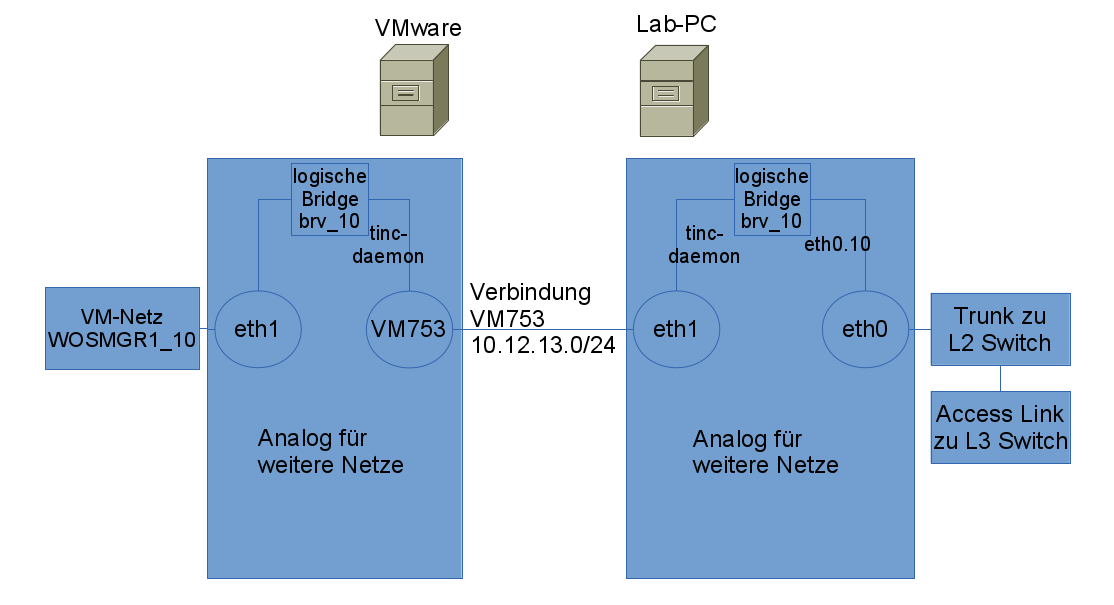
\includegraphics[width=0.8\textwidth]{Phase2/tinc_netz.png}
\caption{Tinc Funktionsweise / Aufbau}
\label{fig:tinc}
\end{figure}

\subsubsection{Konfiguration auf VMware-Umgebung}
Die VM, welche auf VMware-Seite die Tinc-Tunnels terminiert wird als einzige in das vorbereitete VM753-Netz verbunden. Pro VLAN wird auf dem virtuellen VMware-Switch eine zusätzliche Portgruppe definiert. In diese Portgruppe werden dann sowohl die VMs des jeweiligen Netzes als auch ein Interface der Tunnel-VM konfiguriert. Einen Auszug der Netzwerkkonfiguration zeigen die Abbildungen \ref{fig:tinc-esx-overview} und \ref{fig:tinc-esx-tunvm}.

\begin{figure}[H]
\centering
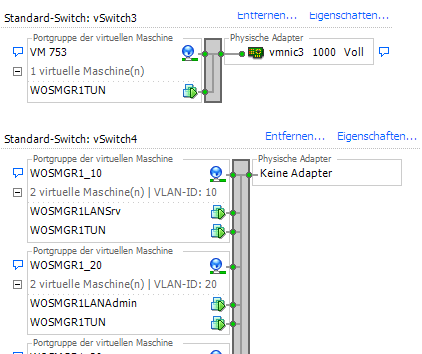
\includegraphics[width=0.7\textwidth]{Phase2/tinc_esx_netz.png}
\caption{Netze auf VMware-Umgebung}
\label{fig:tinc-esx-overview}
\end{figure}

\begin{figure}[H]
\centering
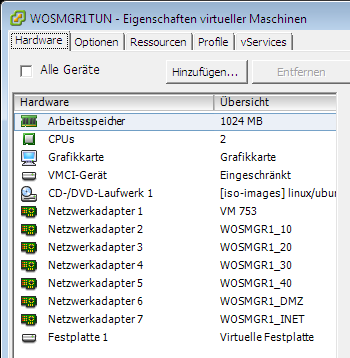
\includegraphics[width=0.5\textwidth]{Phase2/tinc_wosmgr1tun.png}
\caption{Netzwerkkonfiguration Tunnel-VM}
\label{fig:tinc-esx-tunvm}
\end{figure}

\subsubsection{Einrichtung der Tinc-Daemons}
Tinc braucht für das Tunnelling einer Verbindung eine Software-Bridge, an die das erstellte Pseudo-Device angeschlossen werden kann. Die Bridge kann unter Linux folgendermassen erstellt werden (Beispiel: VLAN 10 auf der Tunnel-VM auf VMware):

\begin{lstlisting}
brctl addbr brv_10
ifconfig eth1 0.0.0.0
ifconfig brv_10 up
brctl addif brv_10 eth1
ifconfig eth1 up
\end{lstlisting}

Im Konfigurationsverzeichnis des Tunnels (in diesem Beispiel unter /etc/tinc/bridge\_10/) ist danach eine Datei tinc.conf mit folgenden Inhalt zu erstellen:

\begin{lstlisting}
BindToAddress 10.12.13.1 10010
Name = vlan10_esx
Mode = switch
ConnectTo = vlan10_lab
\end{lstlisting}

Der Eintrag hinter \emph{ConnectTo} bezieht sich dabei auf Files, die unter /etc/tinc/bridge\_10/hosts/ abzulegen sind. In diesen Files sind auch RSA-Keys enthalten, der Befehl \emph{tincd -K} kann benutzt werden um RSA-Schlüsselpaare für Tinc zu erzeugen. Die Host-Dateien sehen folgendermassen aus (Beispiel: vlan10\_esx):

\begin{lstlisting}
Address = 10.12.13.1 10010
-----BEGIN RSA PUBLIC KEY-----
MIIBCgKCAQEAwgQKXRxDjyjL89+4qe3YeFYAFtL5ugFkZS8K/Y9h6HK7dkCZcATl
HM1FS+2UuSbgMd8U7zMd33W0KMat5iZfj/08uQO9cTyx/TibbP7HXpIFRJ/BeB5p
sKvR/SjcWRFPHHC+LIUKLbDkx+SvMaEo/PfswVFFw2Xp8MIYHGH4/ow9cqJjeABH
d6KOwUsDeVF/3pgcuoXL2hw1Iem3SRmQds2siRYkn1UyYWmQ2zHXeTdjym30KDMh
s0Nz8QjJrRFQzADjugAiyktviuI7sqwnjbEIsAlPDVU76ObBN/vPTavH9r8nDEF8
iQSVSfXIob8GThsnikVhUTBElAA17DLEaQIDAQAB
-----END RSA PUBLIC KEY-----
\end{lstlisting}

Tinc braucht des Weiteren ein \emph{tinc-ifup} Script, welches nach der Initialisierung des Tunnel-Interfaces ausgeführt wird. Das folgende Beispielt fügt das Tunnel-Interface (\$INTERFACE) der Bridge brv\_10 hinzu:

\begin{lstlisting}
#!/bin/sh
ifconfig $INTERFACE 0.0.0.0
brctl addif brv_10 $INTERFACE
ifconfig $INTERFACE up
\end{lstlisting}

Sind alle diese Vorbereitungen getroffen kann der Tunnel mit dem Befehl \emph{tincd -n bridge\_10} gestartet werden. \emph{bridge\_10} bezieht sich dabei auf das Konfigurationsverzeichnis unterhalb von \emph{/etc/tinc/}.

\subsubsection{Statusausgaben}
Anzeige der virtuellen Bridges und zugehörigen Interfaces (auf VMware-VM):
\begin{lstlisting}
root@WOSMGR1TUN:~# brctl show
bridge name	bridge id		STP enabled	interfaces
brv_10		8000.005056bc0101	no		bridge_10
							eth1
brv_110		8000.005056bc0105	no		bridge_110
							eth5
brv_120		8000.005056bc0106	no		bridge_120
							eth6
brv_20		8000.005056bc0102	no		bridge_20
							eth2
brv_30		8000.005056bc0103	no		bridge_30
							eth3
brv_40		8000.005056bc0104	no		bridge_40
							eth4
\end{lstlisting}

Anzeige der virtuellen Bridges und zugehörigen Interfaces (auf Lab-PC):
\begin{lstlisting}
root@wosmtunlab:~# brctl show
bridge name	bridge id		STP enabled	interfaces
brv_10		8000.000bcdb58e8c	no		bridge_10
							eth0.10
brv_110		8000.000bcdb58e8c	no		bridge_110
							eth0.110
brv_120		8000.000bcdb58e8c	no		bridge_120
							eth0.120
brv_20		8000.000bcdb58e8c	no		bridge_20
							eth0.20
brv_30		8000.000bcdb58e8c	no		bridge_30
							eth0.30
brv_40		8000.000bcdb58e8c	no		bridge_40
							eth0.40
\end{lstlisting}

\subsubsection{VLAN-Subinterfaces unter Linux}
Die zuvor beschriebenen Punkte reichen für die VM unter VMware aus. Für die Installation im Lab ist es hingegen (aufgrund der begrenzten Anzahl Netzwerkschnittstellen) nötig, die verschiedenen VLANs auf einem Kabel als Trunk auf den Switch zu führen. Dazu kennt Linux, sehr ähnlich wie dies bei Cisco-Geräten der Fall ist, Subinterfaces. Das folgende Listing zeigt beispielhaft die Erstellung eines solchen Interfaces (für VLAN 10):

\begin{lstlisting}
ip link add link eth0 name eth0.10 type vlan id 10
\end{lstlisting}

Datenverkehr, der über das \emph{eth0.10} Interface verschickt wird erhält dadurch das VLAN-Tag 10 und Datenverkehr der auf \emph{eth0} mit einem derartigen Tag erhalten wird taucht auf \emph{eth0.10} ohne Tag auf. Die restlichen für Tinc notwendigen Konfigurationsschritte können normal mit diesem VLAN-Subinterface durchgeführt werden.

\subsubsection{Script für Start der Tunnels}
Um die ansonsten manuell auszuführenden Befehle nicht immer von Hand eintippen zu müssen, wurde für die beiden Tunnel-VMs ein Startscript erstellt. Diese sind in den Anhängen \ref{app:tinc-start-esx} und \ref{app:tinc-start-lab} zu finden.

\subsubsection{VLANs und virtuelle Bridges}
Die folgende Tabelle bietet einen Überblick über die verschiedenen Tunnel, die für den Aufbau im Lab eingerichtet wurden.

\begin{longtable}{p{2.5cm}|p{2cm}|p{1.5cm}|p{2cm}|p{2.5cm}|p{2cm}}
	\textbf{Netz} & \textbf{VLAN ID} & \textbf{Bridge} & \textbf{Tunnel} & \textbf{IF VMware} & \textbf{IF Lab}\\
	\hline
	\endfirsthead
	\textbf{Netz} & \textbf{VLAN ID} & \textbf{Virt. Bridge} & \textbf{Tunnelname} & \textbf{IF VMware} & \textbf{IF Lab}\\
	\hline
	\endhead
	\hline
	\multicolumn{2}{l}{\textit{Fortführung auf nächster Seite\ldots}} \\
	\endfoot
	\endlastfoot
	VM753 & n/a & n/a & n/a & eth0 & eth1 \\
	Int. Server & 10 & brv\_10 & bridge\_10 & eth1 & eth0.10 \\
	Admins & 20 & brv\_20 & bridge\_20 & eth2 & eth0.20 \\
	Entwicklung & 30 & brv\_30 & bridge\_30 & eth3 & eth0.30 \\
	Verkauf & 40 & brv\_40 & bridge\_40 & eth4 & eth0.40 \\
	DMZ & 110 & brv\_110 & bridge\_110 & eth5 & eth0.110 \\
	Internet & 120 & brv\_120 & bridge\_120 & eth6 & eth0.120
\end{longtable}
